% ==========================================
% 强化学习概览 - Beamer Slides
% 编译:xelatex -shell-escape main.tex
% ==========================================

\documentclass[aspectratio=169, 11pt]{beamer}


% ---------- 中文支持 ----------
\usepackage{xeCJK}
\setCJKmainfont{Hiragino Sans GB}
\setCJKsansfont{Heiti SC}

% ---------- 主题设置 ----------
\usetheme{metropolis}           % 现代简洁主题
\metroset{
    progressbar=frametitle,     % 进度条在标题栏
    sectionpage=progressbar,    % section页显示进度条
    numbering=fraction          % 页码显示为 n/N
}

% 颜色配置
\definecolor{primary}{RGB}{0, 83, 156}      % 主色:深蓝
\definecolor{accent}{RGB}{230, 126, 34}     % 强调色:橙色
\definecolor{bglight}{RGB}{250, 250, 252}   % 浅背景

\setbeamercolor{frametitle}{bg=primary, fg=white}
\setbeamercolor{progress bar}{fg=accent}
\setbeamercolor{alerted text}{fg=accent}

% ---------- 超链接设置 ----------
\hypersetup{
    colorlinks=true,
    linkcolor=primary,
    urlcolor=primary
}

% ---------- 引号 ----------
\usepackage{csquotes}
\DeclareQuoteStyle{chinese}{"}{"}{'}{'}\setquotestyle{chinese}

% ---------- 数学宏包 ----------
\usepackage{amsmath, amssymb, amsthm}
\usepackage{mathtools}
\usepackage{bm}
\usepackage{cancel}

% ---------- 图表 ----------
\usepackage{graphicx}
\usepackage{tikz}
\usetikzlibrary{shapes, arrows, positioning, calc}
\usepackage{booktabs}

% ---------- 代码 ----------
\usepackage{minted}
\setminted{fontsize=\footnotesize, breaklines}

% ---------- 自定义命令 (与笔记一致) ----------
\newcommand{\E}{\mathbb{E}}
\newcommand{\R}{\mathbb{R}}
\newcommand{\policy}{\pi}
\newcommand{\Val}{V}
\newcommand{\Qval}{Q}
\newcommand{\discount}{\gamma}
\newcommand{\statespace}{\mathcal{S}}
\newcommand{\actionspace}{\mathcal{A}}
\DeclareMathOperator*{\argmax}{argmax}
\DeclareMathOperator*{\argmin}{argmin}

% ---------- 自定义环境 ----------
% 直觉说明框
\newenvironment{intuition}{%
    \begin{alertblock}{直觉}
}{%
    \end{alertblock}
}

% 关键公式框
\newenvironment{keyformula}{%
    \begin{block}{核心公式}
}{%
    \end{block}
}

% ---------- 文档信息 ----------
\title{\centerline{强化学习概览}}
\subtitle{\centerline{Reinforcement Learning: A Quick Tour}}
\author{卢奇 \\ \texttt{luqi.code@gmail.com}}
\date{}
\institute{}

% ==========================================
% 正文开始
% ==========================================
\begin{document}

% ---------- 标题页 ----------
\begin{frame}
    \titlepage
\end{frame}

% ---------- 目录 ----------
\begin{frame}{大纲}
    \tableofcontents
\end{frame}

% ==========================================
% 第一部分:强化学习基础
% ==========================================
\section{强化学习基础}

\begin{frame}{强化学习:核心框架}
    \begin{columns}[T, onlytextwidth]
        \begin{column}{0.60\textwidth}
            \textbf{核心思想}:Agent 通过与环境交互,学习最大化累积奖励的策略

            \vspace{1em}
            \textbf{Markov Decision Process (MDP)}:
            \begin{itemize}\setlength{\itemsep}{3pt}
                \item \alert{Markov 性质}:$P(s_{t+1}, r_t|s_t,a_t) = P(s_{t+1}, r_t|s_{1:t},a_{1:t})$
                \item 给定 $(s_t, a_t)$,下一状态和奖励的分布与历史无关
            \end{itemize}

            \vspace{0.8em}
            \textbf{MDP 五元组} $(\statespace, \actionspace, P, R, \gamma)$:
            \begin{itemize}\setlength{\itemsep}{2pt}
                \item $\statespace$: 状态空间 \quad $\actionspace$: 动作空间
                \item $P(s'|s,a)$: 转移概率 \quad $R(s,a)$: 奖励函数
                \item $\gamma \in [0,1]$: 折扣因子(权衡即时和长期奖励)
            \end{itemize}

            \vspace{0.8em}
            \textbf{RL 与监督学习的区别}:
            \begin{itemize}\setlength{\itemsep}{2pt}
                \item 无标签,只有奖励信号(延迟、稀疏)
                \item 数据非 i.i.d.,由策略决定
                \item 需要探索与利用的平衡
            \end{itemize}
        \end{column}
        \begin{column}{0.38\textwidth}
            \centering
            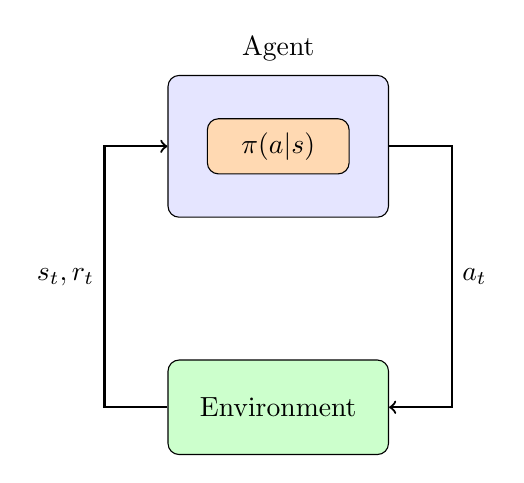
\begin{tikzpicture}[scale=1.0, every node/.style={scale=1.0}]
                \node[draw, rounded corners, fill=blue!10, minimum width=2.8cm, minimum height=1.8cm] (agent) {};
                \node[above=0.05cm of agent.north] {Agent};
                \node[draw, rounded corners, fill=orange!30, minimum width=1.8cm, minimum height=0.7cm] at (agent.center) (policy) {$\policy(a|s)$};
                \node[draw, rounded corners, fill=green!20, minimum width=2.8cm, minimum height=1.2cm, below=1.8cm of agent] (env) {Environment};
                \draw[->, thick] (agent.east) -- ++(0.8,0) |- node[right, pos=0.25] {$a_t$} (env.east);
                \draw[->, thick] (env.west) -- ++(-0.8,0) |- node[left, pos=0.25] {$s_t, r_t$} (agent.west);
            \end{tikzpicture}
        \end{column}
    \end{columns}
\end{frame}

\begin{frame}{交互过程与轨迹(Trajectory)}
    \begin{columns}[T, onlytextwidth]
        \begin{column}{0.65\textwidth}
            \centering
            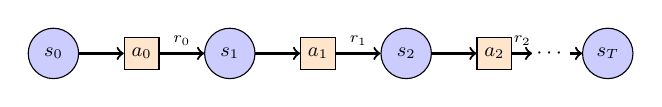
\begin{tikzpicture}[scale=0.8, every node/.style={scale=0.8},
                state/.style={circle, draw, fill=blue!20, minimum size=0.8cm, font=\small},
                action/.style={rectangle, draw, fill=orange!20, minimum size=0.5cm, font=\small}]
                \node[state] (s0) at (0,0) {$s_0$};
                \node[action] (a0) at (1.4,0) {$a_0$};
                \node[state] (s1) at (2.8,0) {$s_1$};
                \node[action] (a1) at (4.2,0) {$a_1$};
                \node[state] (s2) at (5.6,0) {$s_2$};
                \node[action] (a2) at (7.0,0) {$a_2$};
                \node at (7.9,0) {$\cdots$};
                \node[state] (sT) at (8.8,0) {$s_T$};

                \draw[->, thick] (s0) -- (a0);
                \draw[->, thick] (a0) -- node[above] {\scriptsize $r_0$} (s1);
                \draw[->, thick] (s1) -- (a1);
                \draw[->, thick] (a1) -- node[above] {\scriptsize $r_1$} (s2);
                \draw[->, thick] (s2) -- (a2);
                \draw[->, thick] (a2) -- node[above] {\scriptsize $r_2$} (7.6,0);
                \draw[->, thick] (8.2,0) -- (sT);
            \end{tikzpicture}

            \vspace{0.5em}
            \raggedright
            \textbf{轨迹}:$\tau = (s_0, a_0, r_0, s_1, a_1, r_1, \dots, s_T)$

            \vspace{0.3em}
            \alert{Episodic}:有终止 $s_T$(游戏结束) \\
            \alert{Continuing}:$T \to \infty$(无终止状态)

            \vspace{0.8em}
            \textbf{轨迹概率}:$p(\tau|\pi) = p(s_0) \prod_{t=0}^{T-1} \pi(a_t|s_t) \, P(s_{t+1}|s_t,a_t)$

            \vspace{0.8em}
            \textbf{回报}(Return / Reward-to-go):$G_t = \sum_{k=0}^{T-t} \gamma^k r_{t+k}$

            \vspace{0.8em}
            \textbf{目标}:$\pi^* = \argmax_\pi J(\pi)$,其中 $J(\pi) = \E_{\tau \sim \pi}[G_0] = \E_{\tau \sim \pi}\left[\sum_{t=0}^{T} \gamma^t r_t\right]$
        \end{column}
        \begin{column}{0.33\textwidth}
            \textbf{核心符号}

            \vspace{0.4em}
            {\small
            \begin{tabular}{@{}rl@{}}
                $s_t$ & 状态 (state) \\[0.2em]
                $a_t$ & 动作 (action) \\[0.2em]
                $r_t$ & 奖励(即时反馈) \\[0.2em]
                $G_t$ & 回报(累积奖励) \\[0.2em]
                $\pi(a|s)$ & 策略 (policy) \\[0.4em]
                \multicolumn{2}{@{}l}{\textbf{价值函数}} \\[0.2em]
                $\Val^\pi(s)$ & $\E[G_t|s_t{=}s]$ \\[0.1em]
                & 状态价值 \\[0.3em]
                $\Qval^\pi(s,a)$ & $\E[G_t|s_t{=}s,a_t{=}a]$ \\[0.1em]
                & 动作价值 \\
            \end{tabular}
            }
        \end{column}
    \end{columns}
\end{frame}


\begin{frame}{策略与价值函数:怎么评价一条策略?}
    \begin{columns}[T, onlytextwidth]
        \begin{column}{0.63\textwidth}
            \textbf{策略(Policy)}:Agent 在每个状态下选择动作的规则,RL 目标是\alert{找到最优策略 $\pi^*$}

            \vspace{0.5em}
            \textbf{状态价值函数}:从状态 $s$ 出发,在策略 $\pi$ 下的期望回报
            \[V^\pi(s) = \E_\pi [ G_t \mid S_t = s ]\]

            \vspace{0.3em}
            \textbf{动作价值函数}:在 $s$ 采取 $a$,之后遵循 $\pi$ 的期望回报
            \[Q^\pi(s,a) = \E_\pi [ G_t \mid S_t = s, A_t = a ]\]

            \vspace{0.3em}
            \textbf{优势函数}:$A^\pi(s,a) = Q^\pi(s,a) - V^\pi(s)$\\
            衡量动作相对于平均水平的好坏
        \end{column}
        \begin{column}{0.35\textwidth}
            \centering
            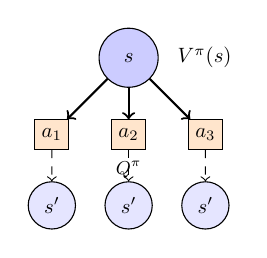
\begin{tikzpicture}[scale=0.75, every node/.style={scale=0.75}]
                \node[circle, draw, fill=blue!20, minimum size=1cm] (s) at (0,0) {$s$};
                \node[rectangle, draw, fill=orange!20, minimum size=0.5cm] (a1) at (-1.3,-1.3) {$a_1$};
                \node[rectangle, draw, fill=orange!20, minimum size=0.5cm] (a2) at (0,-1.3) {$a_2$};
                \node[rectangle, draw, fill=orange!20, minimum size=0.5cm] (a3) at (1.3,-1.3) {$a_3$};
                \draw[->, thick] (s) -- (a1);
                \draw[->, thick] (s) -- (a2);
                \draw[->, thick] (s) -- (a3);
                \node[circle, draw, fill=blue!10, minimum size=0.8cm] (s1) at (-1.3,-2.5) {$s'$};
                \node[circle, draw, fill=blue!10, minimum size=0.8cm] (s2) at (0,-2.5) {$s'$};
                \node[circle, draw, fill=blue!10, minimum size=0.8cm] (s3) at (1.3,-2.5) {$s'$};
                \draw[->, dashed] (a1) -- (s1);
                \draw[->, dashed] (a2) -- (s2);
                \draw[->, dashed] (a3) -- (s3);
                \node[right=0.15cm of s] {$V^\pi(s)$};
                \node[below=0.05cm of a2] {\small $Q^\pi$};
            \end{tikzpicture}

            \vspace{0.5em}
            {\small
            $V^\pi(s)$:状态 $s$ 下的期望回报\\[0.2em]
            $Q^\pi(s,a)$:在 $s$ 执行 $a$ 的期望回报
            }
        \end{column}
    \end{columns}
\end{frame}


% ==========================================
% 第二部分:Value-Based RL
% ==========================================
\section{基于价值的方法}

\begin{frame}{价值函数的递推关系(Bellman 方程)}
    \begin{columns}[T, onlytextwidth]
        \begin{column}{0.62\textwidth}
            \textbf{Bellman Expectation(策略 $\pi$ 下)}
            \[
                \Val^\pi(s) = \E_\pi\big[ r_t + \gamma \Val^\pi(S_{t+1}) \mid S_t = s \big]
            \]
            \[
                \Qval^\pi(s,a) = \E_\pi\big[ r_t + \gamma \Qval^\pi(S_{t+1}, A_{t+1}) \mid S_t{=}s, A_t{=}a \big]
            \]

            \vspace{0.5em}
            \textbf{Bellman Optimality(最优策略 $\pi^*$)}
            \[
                \Val^*(s) = \max_a \E\big[ r_t + \gamma \Val^*(S_{t+1}) \mid S_t{=}s, A_t{=}a \big]
            \]
            \[
                \Qval^*(s,a) = \E\big[ r_t + \gamma \max_{a'} \Qval^*(S_{t+1}, a') \mid S_t{=}s, A_t{=}a \big]
            \]
            {\small 最优价值 = 选最好的动作后能获得的期望回报\\
            后面 Q-Learning / DQN 就是基于 $\Qval^*$ 这个式子}

        \end{column}
        \begin{column}{0.36\textwidth}
            \centering
            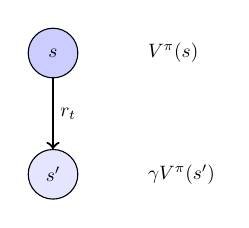
\begin{tikzpicture}[scale=0.7, every node/.style={scale=0.7}]
                \node[circle, draw, fill=blue!20, minimum size=0.9cm] (s) at (0,0) {$s$};
                \node[circle, draw, fill=blue!10, minimum size=0.9cm] (s1) at (0,-2.2) {$s'$};
                \draw[->, thick] (s) -- node[right] {$r_t$} (s1);
                \node[right=0.8cm of s] {$\Val^\pi(s)$};
                \node[right=0.8cm of s1] {$\gamma \Val^\pi(s')$};
            \end{tikzpicture}

            \vspace{0.5em}
            {\small
            \alert{直觉}:\\
            今天的价值 =\\
            这一步奖励 $r_t$ +\\
            折扣后的明天 $\gamma \Val^\pi(s')$
            }
        \end{column}
    \end{columns}
\end{frame}

\begin{frame}{如何用样本估计价值函数:MC vs TD}
    \begin{columns}[T, onlytextwidth]
        \begin{column}{0.48\textwidth}
            \textbf{Monte Carlo (MC)}
            \[
                V(S_t) \leftarrow V(S_t) + \alpha \big( \alert{G_t} - V(S_t) \big)
            \]
            \begin{itemize}\setlength{\itemsep}{2pt}
                \item 用完整回报 $G_t = \sum_{k=0}^{T-t} \gamma^k r_{t+k}$
                \item 必须等 episode 结束(对 episodic 任务)
                \item \alert{无偏}:因为是直接对目标进行优化,期望是一样,但\alert{方差大}:因为mc是针对单条轨迹的,同一个策略不同轨迹天然回报差异就比较大
                \item 不 bootstrap(目标完全来自真实采样回报)
            \end{itemize}
        \end{column}
        \begin{column}{0.48\textwidth}
            \textbf{Temporal Difference (TD)}
            \[
                V(S_t) \leftarrow V(S_t) + \alpha \big( \alert{r_t + \gamma V(S_{t+1})} - V(S_t) \big)
            \]
            \begin{itemize}\setlength{\itemsep}{2pt}
                \item 用单步估计 $r_t + \gamma V(S_{t+1})$
                \item 每步都能更新(可在线学习)
                \item 有偏(目标中用了 $V(S_{t+1})$ 的估计),但\alert{方差小}:V是一个相对比较平滑的函数
                \item Bootstrap:用自己的估计去更新估计
            \end{itemize}
        \end{column}
    \end{columns}
\end{frame}

\begin{frame}{Q-Learning vs SARSA:Off-policy 与 On-policy}
    \textbf{核心思想}:不再评估某条给定策略 $\Qval^\pi$,而是以 Bellman Optimality 为目标,\alert{直接逼近最优 $\Qval^*$}

    \vspace{0.3em}
    \begin{columns}[T, onlytextwidth]
        \begin{column}{0.48\textwidth}
            \textbf{Q-Learning}(Off-policy)
            {\small
            \[
                \Qval(s_t, a_t) \!\leftarrow\! \Qval + \alpha \big( r_t {+} \gamma \alert{\max_{a'}} \Qval(s_{t+1}, a') {-} \Qval \big)
            \]}
            \vspace{-0.5em}
            \begin{itemize}\setlength{\itemsep}{1pt}
                \item 目标用 $\max_{a'}$:直接逼近 $\Qval^*$
                \item 行为策略和目标策略\alert{可以不同}
                \item 更激进,样本效率高
            \end{itemize}
        \end{column}
        \begin{column}{0.48\textwidth}
            \textbf{SARSA}(On-policy)
            {\small
            \[
                \Qval(s_t, a_t) \!\leftarrow\! \Qval + \alpha \big( r_t {+} \gamma \Qval(s_{t+1}, \alert{a_{t+1}}) {-} \Qval \big)
            \]}
            \vspace{-0.5em}
            \begin{itemize}\setlength{\itemsep}{1pt}
                \item 目标用实际采样的 $a_{t+1}$:学习 $\Qval^\pi$
                \item 行为策略和目标策略\alert{必须相同}
                \item 更保守,考虑探索代价
            \end{itemize}
        \end{column}
    \end{columns}

    \vspace{0.3em}
    \textbf{$\epsilon$-greedy 探索}:以 $1{-}\epsilon$ 概率选 $\arg\max_a \Qval$,以 $\epsilon$ 概率随机 \quad {\small(其他:UCB、Softmax、Boltzmann)}

    \vspace{0.2em}
    {\small \textbf{后续}:DQN = Q-Learning + 神经网络 + Experience Replay + Target Network}
\end{frame}

\begin{frame}{DQN:用神经网络逼近 $\Qval^*$}
    \textbf{问题}:表格 Q-Learning 无法处理大状态空间(如图像输入、连续状态),也难以泛化到没见过的状态

    \vspace{0.4em}
    \textbf{解决}:用神经网络 $\Qval(s,a;\theta)$ 逼近 $\Qval^*$,最小化 TD 误差
    \[
        \mathcal{L}(\theta) = \E\Big[\big( \underbrace{r_t + \gamma \max_{a'} \Qval(s_{t+1}, a'; \theta^-)}_{\text{TD target}} - \Qval(s_t,a_t;\theta) \big)^2\Big]
    \]

    \vspace{0.4em}
    \begin{columns}[T, onlytextwidth]
        \begin{column}{0.48\textwidth}
            \textbf{Experience Replay}
            \begin{itemize}\setlength{\itemsep}{2pt}
                \item 将 $(s_t,a_t,r_t,s_{t+1})$ 存入 buffer
                \item 随机采样 mini-batch 训练
                \item 打破样本相关性,提高数据效率
            \end{itemize}
        \end{column}
        \begin{column}{0.48\textwidth}
            \textbf{Target Network}
            \begin{itemize}\setlength{\itemsep}{2pt}
                \item 用 $\theta^-$(旧参数)计算 target
                \item 定期更新 $\theta^- \leftarrow \theta$
                \item 稳定训练,避免目标\enquote{互相追着跑}
            \end{itemize}
        \end{column}
    \end{columns}

    \vspace{0.5em}
    \textbf{DQN 变体}:Double DQN(解耦选动作与估值)、Dueling DQN(分离 $\Val$ 和 $\Qval$)、Rainbow...
\end{frame}

% ==========================================
% 第三部分:Policy-Based RL
% ==========================================
\section{基于策略的方法}

\begin{frame}{Value-Based 的局限与 Policy-Based 的动机}
    \begin{columns}[T, onlytextwidth]
        \begin{column}{0.48\textwidth}
            \textbf{Value-Based 的局限}
            \begin{itemize}\setlength{\itemsep}{3pt}
                \item \alert{连续动作困难}:$\max_a \Qval(s,a)$ 需要枚举所有动作,连续动作空间无法直接处理
                \item \alert{函数逼近不稳定}:Deadly Triad——函数逼近 + Bootstrapping + Off-policy 同时使用时容易发散
                \item \alert{目标不直接}:通过最小化 TD 误差来逼近 Bellman 方程的解,而非期望回报 $J(\pi)$
                \item \alert{只能学确定性策略}:$\arg\max$ 输出确定动作,但在随机/部分可观测环境中,随机策略更优
            \end{itemize}
        \end{column}
        \begin{column}{0.48\textwidth}
            \textbf{Policy-Based:直接优化策略参数}

            \vspace{0.3em}
            用参数化策略 $\pi_\theta(a|s)$(通常是神经网络),直接最大化期望回报:
            \[
                J(\theta) = \E_{\tau \sim \pi_\theta}[G_0]
            \]

            \vspace{0.3em}
            \textbf{策略输出形式}:
            \begin{itemize}\setlength{\itemsep}{2pt}
                \item 离散动作:softmax → Categorical 分布
                \item 连续动作:输出 $\mu, \sigma$ → Gaussian 分布
            \end{itemize}

            \vspace{0.3em}
            \textbf{核心问题}:如何计算 $\nabla_\theta J(\theta)$?
        \end{column}
    \end{columns}
\end{frame}

\begin{frame}{Policy Gradient 定理推导}
    \textbf{目标}:最大化期望回报 $J(\theta) = \E_{\tau \sim \pi_\theta}[G_0]$,其中 $G_0 = \sum_{t=0}^{T} \gamma^t r_t$(Return)

    \vspace{0.3em}
    \textbf{推导}:记 $R(\tau) = G_0$,轨迹概率 $p(\tau|\theta) = p(s_0) \prod_{t} \pi_\theta(a_t|s_t) P(s_{t+1}|s_t,a_t)$
    \begin{align*}
        \nabla_\theta J(\theta) &= \nabla_\theta \int p(\tau|\theta) R(\tau) d\tau = \int p(\tau|\theta) \nabla_\theta \log p(\tau|\theta) R(\tau) d\tau \\
        &= \E_{\tau \sim \pi_\theta}\left[ \nabla_\theta \log p(\tau|\theta) \cdot R(\tau) \right] \quad \text{(Log-derivative trick)}
    \end{align*}

    \textbf{关键}:$\nabla_\theta \log p(\tau|\theta) = \sum_{t} \nabla_\theta \log \pi_\theta(a_t|s_t)$(环境动力学 $P$ 与 $\theta$ 无关!)

    \vspace{0.4em}
    \textbf{Policy Gradient Theorem}:
    \[
        \boxed{\nabla_\theta J(\theta) = \E_{\tau \sim \pi_\theta}\left[ \sum_{t=0}^{T} \nabla_\theta \log \pi_\theta(a_t|s_t) \cdot G_t \right]}
    \]
    其中 reward-to-go $G_t = \sum_{k=0}^{T-t} \gamma^{k} r_{t+k}$(从 $t$ 时刻开始的折扣回报)
\end{frame}

\begin{frame}{REINFORCE:蒙特卡洛策略梯度}
    \textbf{REINFORCE 算法}:用采样轨迹估计策略梯度
    \[
        \nabla_\theta J(\theta) \approx \frac{1}{N} \sum_{i=1}^{N} \sum_{t=0}^{T} \nabla_\theta \log \pi_\theta(a_t^{(i)}|s_t^{(i)}) \cdot G_t^{(i)}
    \]

    \vspace{0.5em}
    \begin{columns}[T, onlytextwidth]
        \begin{column}{0.48\textwidth}
            \textbf{为什么是无偏的?}
            \begin{itemize}\setlength{\itemsep}{3pt}
                \item $G_t$ 是真实回报的采样
                \item 期望 $\E[G_t | s_t, a_t] = \Qval^\pi(s_t, a_t)$
                \item 采样均值 → 期望(大数定律)
                \item 不依赖任何函数逼近
            \end{itemize}
        \end{column}
        \begin{column}{0.48\textwidth}
            \textbf{为什么方差大?}
            \begin{itemize}\setlength{\itemsep}{3pt}
                \item $G_t$ 累积了整条轨迹的随机性
                \item 环境随机 + 策略随机 → 方差叠加
                \item 轨迹越长,方差越大
                \item 奖励稀疏时,$G_t$ 变化剧烈
            \end{itemize}
        \end{column}
    \end{columns}

    \vspace{0.6em}
    \textbf{直觉}:$G_t$ 包含了很多与当前动作 $a_t$ 无关的噪声(未来的随机事件),但都被算进了梯度

    \vspace{0.4em}
    {\small \textbf{下一步}:如何降低方差?→ Baseline / Advantage / Actor-Critic}
\end{frame}

\begin{frame}{降低方差:Baseline}
    \textbf{问题}:REINFORCE 方差太大,能否在不改变期望的情况下降低方差?

    \vspace{0.4em}
    \textbf{Baseline 技巧}:减去任意只依赖于 $s$、\alert{不依赖动作 $a$} 的 baseline $b(s)$
    \[
        \nabla_\theta J(\theta) = \E\left[ \sum_{t} \nabla_\theta \log \pi_\theta(a_t|s_t) \cdot (G_t - b(s_t)) \right]
    \]

    \textbf{为什么可以减?} $\E_{a \sim \pi}[\nabla_\theta \log \pi_\theta(a|s) \cdot b(s)] = b(s) \cdot \nabla_\theta \underbrace{\sum_a \pi_\theta(a|s)}_{=1} = 0$

    \vspace{0.5em}
    \textbf{最优 baseline}:在不改变期望的前提下,$b(s) = \Val^\pi(s)$ 可证明使方差最小

    \vspace{0.3em}
    {\small 回顾:$\Val^\pi(s) = \E_\pi[G_t | S_t = s]$,即从状态 $s$ 出发的期望回报}

    \vspace{0.5em}
    \textbf{直觉}:$G_t$ 包含\enquote{基线}(状态本身好坏),减去 $\Val^\pi(s)$ 后只剩动作带来的增益
\end{frame}

\begin{frame}{Advantage Function}
    当 $b(s) = \Val^\pi(s)$ 时,$G_t - \Val^\pi(s_t)$ 的期望是什么?在给定 $(s, a)$ 条件下:
    \[
        \E_\pi[G_t - \Val^\pi(s) \mid S_t = s, A_t = a] = \Qval^\pi(s, a) - \Val^\pi(s)
    \]

    定义 \alert{Advantage Function}:$\boxed{A^\pi(s,a) = \Qval^\pi(s,a) - \Val^\pi(s)}$

    \vspace{0.5em}
    \begin{columns}[T, onlytextwidth]
        \begin{column}{0.55\textwidth}
            \textbf{三个价值函数对比}:
            \begin{itemize}\setlength{\itemsep}{4pt}
                \item $\Val^\pi(s) = \E_\pi[G_t | S_t = s]$\\
                      {\small 在 $s$ 按策略 $\pi$ 的期望回报}
                \item $\Qval^\pi(s,a) = \E_\pi[G_t | S_t = s, A_t = a]$\\
                      {\small 在 $s$ 选定动作 $a$ 后的期望回报}
                \item $A^\pi(s,a) = \Qval^\pi(s,a) - \Val^\pi(s)$\\
                      {\small 动作 $a$ 比\enquote{平均}好多少}
            \end{itemize}
        \end{column}
        \begin{column}{0.43\textwidth}
            \textbf{Policy Gradient with Advantage}:
            \[
                \E\big[\nabla_\theta \log \pi_\theta \cdot A^\pi\big]
            \]

            \vspace{0.3em}
            \textbf{$\hat{A}_t$ 的不同估计方式}:
            \begin{itemize}\setlength{\itemsep}{2pt}
                \item MC:$G_t - \Val(s_t)$(无偏,高方差)
                \item TD:$r_t + \gamma \Val(s_{t+1}) - \Val(s_t)$(有偏,低方差)
                \item GAE:介于两者之间
            \end{itemize}
        \end{column}
    \end{columns}
\end{frame}

\begin{frame}{Actor-Critic}
    \textbf{核心思想}:同时学习 Actor(策略 $\pi_\theta$)和 Critic(价值函数 $\hat{\Val}_\phi$)

    \vspace{0.4em}
    \begin{columns}[T, onlytextwidth]
        \begin{column}{0.55\textwidth}
            \textbf{Actor}(策略网络):
            \begin{itemize}\setlength{\itemsep}{3pt}
                \item 输出动作分布 $\pi_\theta(a|s)$
                \item 用 Policy Gradient 更新:
                      $\theta \leftarrow \theta + \alpha \nabla_\theta \log \pi_\theta \cdot \hat{A}_t$
            \end{itemize}

            \vspace{0.3em}
            \textbf{Critic}(价值网络):
            \begin{itemize}\setlength{\itemsep}{3pt}
                \item 估计 $\hat{\Val}_\phi(s) \approx \Val^\pi(s)$
                \item 回归到 return 或 TD target:
                      $L_V(\phi) = \E[(G_t - \Val_\phi(s_t))^2]$ 或 $\E[\delta_t^2]$
            \end{itemize}
        \end{column}
        \begin{column}{0.42\textwidth}
            \textbf{训练循环}:\\[0.3em]
            \centering
            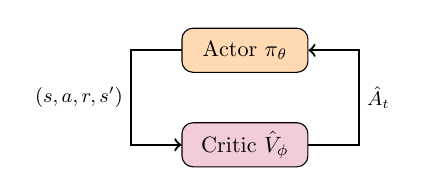
\begin{tikzpicture}[scale=0.8, every node/.style={scale=0.8},
                box/.style={draw, rounded corners, minimum width=2cm, minimum height=0.7cm}]
                \node[box, fill=orange!30] (actor) at (0, 0) {Actor $\pi_\theta$};
                \node[box, fill=purple!20] (critic) at (0, -1.5) {Critic $\hat{\Val}_\phi$};
                \draw[->, thick] (critic.east) -- ++(0.8,0) |- node[right, pos=0.25, font=\small] {$\hat{A}_t$} (actor.east);
                \draw[->, thick] (actor.west) -- ++(-0.8,0) |- node[left, pos=0.25, font=\small] {$(s,a,r,s')$} (critic.west);
            \end{tikzpicture}

            \vspace{0.5em}
            \raggedright
            \textbf{为什么需要 Critic?}
            \begin{itemize}\setlength{\itemsep}{2pt}
                \item 提供 $\hat{\Val}(s)$ 计算 $\hat{A}_t$
                \item 比纯 MC ($G_t$) 方差更小
                \item 可每步更新,不用等 episode 结束
            \end{itemize}
        \end{column}
    \end{columns}
\end{frame}

\begin{frame}{GAE:Generalized Advantage Estimation}
    \textbf{问题}:MC 估计 $\hat{A}_t = G_t - \hat{\Val}(s_t)$(相对无偏,方差大),TD 估计 $\hat{A}_t = \delta_t$(方差小,但有偏)

    \vspace{0.3em}
    \textbf{GAE 思路}:用 $\lambda \in [0,1]$ 插值,定义 TD 残差 $\delta_t = r_t + \gamma \hat{\Val}(s_{t+1}) - \hat{\Val}(s_t)$
    \[
        \hat{A}_t^{\text{GAE}} = \sum_{l=0}^{\infty} (\gamma \lambda)^l \delta_{t+l} = \delta_t + \gamma\lambda \delta_{t+1} + (\gamma\lambda)^2 \delta_{t+2} + \cdots
    \]

    \vspace{0.2em}
    \begin{columns}[T, onlytextwidth]
        \begin{column}{0.48\textwidth}
            \textbf{$\lambda$ 的作用}:
            \begin{itemize}\setlength{\itemsep}{2pt}
                \item $\lambda = 0$:单步 TD,$\hat{A}_t = \delta_t$(偏差大,方差小)
                \item $\lambda = 1$:等价 MC,$\hat{A}_t = G_t - \hat{\Val}(s_t)$(相对无偏,方差大)
                \item $\lambda \in (0,1)$:bias-variance tradeoff,常用 $\lambda = 0.95$
            \end{itemize}
        \end{column}
        \begin{column}{0.48\textwidth}
            \textbf{直觉}:
            \begin{itemize}\setlength{\itemsep}{2pt}
                \item $\delta_t$ 是单步 advantage 估计
                \item GAE 把多步 $\delta$ 加权求和
                \item $(\gamma\lambda)^l$ 让远处 $\delta$ 权重指数衰减
                \item 类似 TD($\lambda$) 的思想
            \end{itemize}

            \vspace{0.2em}
            {\small PPO、TRPO 等算法都使用 GAE}
        \end{column}
    \end{columns}
\end{frame}

\begin{frame}{重要性采样:提高样本效率}
    \textbf{问题}:Policy Gradient 是 on-policy 的——每次更新 $\theta$ 后,旧数据就\enquote{过期}了,样本效率低

    \vspace{0.3em}
    \textbf{重要性采样}(Importance Sampling):用旧策略 $\pi_{\text{old}}$ 的样本,估计新策略 $\pi_\theta$ 下的期望

    \vspace{0.3em}
    \textbf{推导}(为什么不改变期望):
    \begin{align*}
        \E_{a \sim \pi_\theta}[f(a)] &= \sum_a \pi_\theta(a) f(a) = \sum_a \pi_{\text{old}}(a) \cdot \frac{\pi_\theta(a)}{\pi_{\text{old}}(a)} f(a) \\
        &= \E_{a \sim \pi_{\text{old}}}\left[\frac{\pi_\theta(a)}{\pi_{\text{old}}(a)} f(a)\right]
    \end{align*}

    \vspace{0.3em}
    \textbf{应用到 Policy Gradient}:记重要性权重 $\rho_t(\theta) = \frac{\pi_\theta(a_t|s_t)}{\pi_{\text{old}}(a_t|s_t)}$
    \[
        \nabla_\theta J(\theta) = \E_{\pi_{\text{old}}}\left[ \rho_t(\theta) \nabla_\theta \log \pi_\theta(a_t|s_t) \hat{A}_t \right]
    \]

    {\small 可以复用旧数据多次更新!但 $\rho_t$ 偏离 1 太多时方差会变大 → 需要限制更新幅度}
\end{frame}

\begin{frame}{PPO:Proximal Policy Optimization}
    \textbf{问题}:重要性采样后,$\rho_t(\theta)$ 偏离 1 太多会导致方差爆炸、策略崩溃

    \vspace{0.4em}
    \textbf{解决思路}:限制策略更新幅度,让 $\rho_t$ 不要偏离 1 太远

    \vspace{0.3em}
    \begin{columns}[T, onlytextwidth]
        \begin{column}{0.48\textwidth}
            \textbf{TRPO}:KL 散度约束
            \[
                \max_\theta \E[\rho_t \hat{A}_t]
            \]
            \[
                \text{s.t.} \quad \text{KL}(\pi_{\text{old}} \| \pi_\theta) \leq \delta
            \]
            {\small 理论优美,但需二阶优化,实现复杂}
        \end{column}
        \begin{column}{0.48\textwidth}
            \textbf{PPO-Clip}:截断重要性权重
            \[
                L^{\text{CLIP}} = \E\big[\min(\rho_t \hat{A}_t, \text{clip}(\rho_t, 1{\pm}\epsilon) \hat{A}_t)\big]
            \]
            {\small 简单高效,一阶优化,常用 $\epsilon = 0.2$}

            \vspace{0.3em}
            \textbf{PPO-KL}:KL 惩罚项
            \[
                L = \E[\rho_t \hat{A}_t] - \beta \cdot \text{KL}
            \]
            {\small 自适应调整 $\beta$}
        \end{column}
    \end{columns}
\end{frame}

% ==========================================
% 第四部分:Model-Based RL & Multi-Agent RL
% ==========================================
\section{Model-Based 与 Multi-Agent}

\begin{frame}{Model-Based RL \& Multi-Agent RL}
    \begin{columns}[T, onlytextwidth]
        \begin{column}{0.48\textwidth}
            \textbf{Model-Based RL}:\alert{利用/学习}环境模型

            \vspace{0.2em}
            \textbf{核心}:得到 $\hat{P}(s'|s,a)$, $\hat{R}(s,a)$(已知规则或学习),在模型中规划

            \vspace{0.2em}
            \textbf{两种用法}:
            \begin{itemize}\setlength{\itemsep}{1pt}
                \item \textbf{Background Planning}:模型生成数据训练
                \item \textbf{Decision-time Planning}:向前搜索(MCTS)
            \end{itemize}

            \vspace{0.2em}
            \textbf{优势}:样本效率高,可在\enquote{想象}中学习

            \textbf{劣势}:模型不准 → \alert{model bias}
        \end{column}
        \begin{column}{0.48\textwidth}
            \textbf{Multi-Agent RL}:多智能体博弈

            \vspace{0.2em}
            \textbf{与单智能体的区别}:
            \begin{itemize}\setlength{\itemsep}{1pt}
                \item 环境包含其他 agent(\alert{非稳态})
                \item 需要考虑对手/队友策略变化
                \item 博弈论常用 \alert{Nash 均衡} 描述稳定解
            \end{itemize}

            \vspace{0.2em}
            \textbf{两种设定}:
            \begin{itemize}\setlength{\itemsep}{1pt}
                \item \textbf{合作}:最大化团队收益
                \item \textbf{竞争/零和}:一方获益 = 另一方损失
            \end{itemize}

            \vspace{0.2em}
            \textbf{Self-Play}:与自己(历史版本)博弈,不断提升
        \end{column}
    \end{columns}

    \vspace{0.3em}
    \textbf{AlphaZero} 可以看作:Model-Based(已知棋规 + MCTS)+ Multi-Agent(自我对弈)
\end{frame}

\begin{frame}{AlphaGo / AlphaZero:MCTS + 深度学习}
    \begin{columns}[T, onlytextwidth]
        \begin{column}{0.48\textwidth}
            \textbf{AlphaGo}(2016,击败李世石):
            \begin{itemize}\setlength{\itemsep}{1pt}
                \item \textbf{Policy Network}:人类棋谱监督预训练
                \item \textbf{Policy Gradient}:自我对弈强化
                \item \textbf{Value Network}:预测胜率
                \item \textbf{MCTS}:结合 $p_\theta$, $v_\phi$ 搜索
            \end{itemize}

            \vspace{0.2em}
            \textbf{MCTS 四步}:Selection(UCB)→ Expansion($p_\theta$)→ Evaluation($v_\phi$)→ Backup
        \end{column}
        \begin{column}{0.48\textwidth}
            \textbf{AlphaZero}(改进):
            \begin{itemize}\setlength{\itemsep}{1pt}
                \item \alert{不需要人类棋谱}:从零自我对弈
                \item \alert{统一网络}:同时输出 $p_\theta$, $v_\phi$
                \item \alert{更简洁}:去掉 rollout
            \end{itemize}

            \vspace{0.2em}
            \textbf{训练循环}:
            \begin{enumerate}\setlength{\itemsep}{0pt}
                \item 网络 + MCTS 自我对弈
                \item 记录 $(s, \pi_{\text{MCTS}}, z)$
                \item $p_\theta \to \pi_{\text{MCTS}}$,$v_\phi \to z$
                \item 重复,越来越强
            \end{enumerate}
        \end{column}
    \end{columns}

    \vspace{0.3em}
    \textbf{核心循环}:MCTS 改进策略 → 网络学习搜索结果 → 更强网络 → 自我对弈生成无限数据
\end{frame}

% ==========================================
% 第五部分:LLM 与强化学习
% ==========================================
\section{LLM 与强化学习}

\begin{frame}{LLM 中的 RL:如何建模?}
    \textbf{核心问题}:如何把\enquote{LLM 对齐}建模成 RL 问题?

    \vspace{0.2em}
    \begin{columns}[T, onlytextwidth]
        \begin{column}{0.48\textwidth}
            \textbf{RL 视角下的 LLM}:
            \begin{itemize}\setlength{\itemsep}{1pt}
                \item \textbf{State} $s$:prompt + 已生成的 token 序列
                \item \textbf{Action} $a$:下一个 token(词表 $|\mathcal{V}|$)
                \item \textbf{Policy} $\pi_\theta(a|s)$:LLM 本身
                \item \textbf{Trajectory} $\tau$:完整的生成序列
                \item \textbf{Reward} $r$:只在序列结束时给出
            \end{itemize}

            \vspace{0.2em}
            \textbf{特点}:
            \begin{itemize}\setlength{\itemsep}{1pt}
                \item 动作空间巨大(词表 $\sim$100k)
                \item \alert{稀疏奖励}:只有最后一步有 reward
                \item Episode = 一次完整生成
            \end{itemize}
        \end{column}
        \begin{column}{0.48\textwidth}
            \textbf{RLHF 优化目标}:

            \vspace{0.2em}
            \textbf{Reward Model}:学习人类偏好
            \begin{itemize}\setlength{\itemsep}{1pt}
                \item 人类标注偏好对:$y_w \succ y_l$
            \end{itemize}

            \vspace{0.2em}
            \textbf{目标函数}:
            \[
                \max_\theta \E_{y \sim \pi_\theta}\big[r_\phi(x,y)\big] - \beta \text{KL}(\pi_\theta \| \pi_{\text{ref}})
            \]

            \begin{itemize}\setlength{\itemsep}{1pt}
                \item $r_\phi(x,y)$:Reward Model 打分
                \item $\text{KL}(\pi_\theta \| \pi_{\text{ref}})$:约束项
                \item $\pi_{\text{ref}}$:SFT 后的初始模型
            \end{itemize}

            \vspace{0.2em}
            {\small KL 项可以稳定训练,防止模型\enquote{hack} reward model}
        \end{column}
    \end{columns}
\end{frame}

\begin{frame}{RLHF:三阶段流程与 PPO 更新}
    \begin{columns}[T, onlytextwidth]
        \begin{column}{0.53\textwidth}
            \textbf{Stage 1: Supervised Fine-Tuning (SFT)}
            \begin{itemize}\setlength{\itemsep}{0pt}
                \item 用高质量对话数据微调预训练模型
                \item 得到参考模型 $\pi_{\text{ref}}$
            \end{itemize}

            \vspace{0.25em}
            \textbf{Stage 2: Reward Model 训练}
            \begin{itemize}\setlength{\itemsep}{0pt}
                \item 收集人类偏好数据 $(x, y_w, y_l)$
                \item Bradley-Terry pairwise loss:
                \vspace{-0.3em}
                \[
                    L(\phi) = -\E\big[\log \sigma(r_\phi(x,y_w) - r_\phi(x,y_l))\big]
                \]
            \end{itemize}

            \vspace{0.1em}
            \textbf{Stage 3: 用 PPO 微调策略}
            \begin{itemize}\setlength{\itemsep}{0pt}
                \item 用 $r_\phi$ 提供奖励信号
                \item 优化\enquote{高奖励 + 小 KL}目标
                \item 使用 Advantage / GAE + PPO-Clip
            \end{itemize}
        \end{column}
        \begin{column}{0.45\textwidth}
            \textbf{PPO 更新步骤}:
            \begin{enumerate}\setlength{\itemsep}{0pt}
                \item 用 $\pi_{\theta_{\text{old}}}$ 生成回复 $y$
                \item 计算序列总奖励:
                \vspace{-0.3em}
                \[
                    R = r_\phi(x,y) - \beta \log \frac{\pi_{\theta_{\text{old}}}(y|x)}{\pi_{\text{ref}}(y|x)}
                \]
                \vspace{-0.5em}
                \item 用 GAE 计算 $\hat{A}_t$
                \item 计算比率 $\rho_t(\theta) = \frac{\pi_\theta(a_t|s_t)}{\pi_{\theta_{\text{old}}}(a_t|s_t)}$
            \end{enumerate}

            \vspace{0.2em}
            \textbf{PPO-Clip 目标}:
            \vspace{-0.3em}
            \[
                L^{\text{CLIP}} = \E\big[\min(\rho_t \hat{A}_t, \text{clip}(\rho_t, 1{\pm}\epsilon) \hat{A}_t)\big]
            \]

            {\small 总 loss = 策略 + 值函数 + 熵正则}
        \end{column}
    \end{columns}
\end{frame}

\begin{frame}{DPO:绕过 Reward Model 和 PPO}
    \textbf{DPO Loss}:
    \vspace{-0.3em}
    \[
        \boxed{
        L_{\text{DPO}}(\theta) = -\E_{(x, y_w, y_l)}\Big[
            \log \sigma\Big(
                \beta\big[
                    \log \frac{\pi_\theta(y_w|x)}{\pi_{\text{ref}}(y_w|x)}
                  - \log \frac{\pi_\theta(y_l|x)}{\pi_{\text{ref}}(y_l|x)}
                \big]
            \Big)
        \Big]
        }
    \]

    \vspace{0.2em}
    \begin{columns}[T, onlytextwidth]
        \begin{column}{0.48\textwidth}
            \textbf{RLHF + PPO 的问题}:
            \begin{itemize}\setlength{\itemsep}{1pt}
                \item 需要维护 $\pi_\theta$、$V_\psi$、$r_\phi$ 三个模型
                \item 在线采样成本高(大模型生成贵)
                \item PPO 超参敏感,实现不稳定
            \end{itemize}

            \vspace{0.3em}
            \textbf{DPO 的思路}:
            \begin{itemize}\setlength{\itemsep}{1pt}
                \item 直接在偏好数据 $(x, y_w, y_l)$ 上优化
                \item \alert{不需要 Reward Model 和 PPO}
                \item 离线训练,形式像监督学习
            \end{itemize}
        \end{column}
        \begin{column}{0.50\textwidth}
            \textbf{推导思路}(\hyperlink{appendix:dpo}{详见附录 A}):
            \begin{enumerate}\setlength{\itemsep}{1pt}
                \item KL 正则 RL 目标引入配分函数 $Z(x)$
                \item 最优策略:$\pi^*(y|x) \propto \pi_{\text{ref}}(y|x) e^{r(x,y)/\beta}$
                \item 反解:$r^* = \beta \log \frac{\pi^*}{\pi_{\text{ref}}} + \beta \log Z$
                \item 代入 Bradley-Terry,$Z(x)$ 消掉
                \item 最大似然优化 → DPO Loss
            \end{enumerate}

            \vspace{0.3em}
            \textbf{直观理解}:
            \begin{itemize}\setlength{\itemsep}{1pt}
                \item 提高 $y_w$ 相对 $\pi_{\text{ref}}$ 的 log-prob
                \item 压低 $y_l$ 相对 $\pi_{\text{ref}}$ 的 log-prob
            \end{itemize}
        \end{column}
    \end{columns}
\end{frame}

\begin{frame}{GRPO:Group Relative Policy Optimization}
    \begin{columns}[T, onlytextwidth]
        \begin{column}{0.48\textwidth}
            \textbf{动机}:PPO 太重,DPO 又不够用

            \vspace{0.3em}
            \textbf{PPO}:需要 Critic 网络,显存开销大

            \vspace{0.2em}
            \textbf{DPO}:
            \begin{itemize}\setlength{\itemsep}{2pt}
                \item 完全 offline,\alert{没有探索机制}
                \item Pairwise 信号粗糙,不知道好多少
                \item 难任务(数学/代码)提升有限
            \end{itemize}

            \vspace{0.3em}
            \textbf{GRPO 做法}:
            \begin{enumerate}\setlength{\itemsep}{3pt}
                \item 对 prompt $x$,采样一组 $\{y_1,\dots,y_G\}$
                \item 计算组内奖励 $\{R_1,\dots,R_G\}$
                \item 组内标准化:$\hat{A}_i = \frac{R_i - \overline{R}}{\text{Std}(R)}$
                \item PPO-Clip 更新
            \end{enumerate}
        \end{column}
        \begin{column}{0.50\textwidth}
            \textbf{核心}:用\alert{组内相对奖励}代替 Critic

            \vspace{0.2em}
            \textbf{目标函数}:
            \vspace{-0.3em}
            \[
                L_{\text{GRPO}} = \E\!\left[
                    \frac{1}{G} \sum_{i=1}^{G} \sum_t
                    \min\big(
                        \rho_{i,t}\hat{A}_i,
                        \text{clip}(\rho_{i,t})\hat{A}_i
                    \big)
                \right]
            \]
            \vspace{-0.3em}
            {\small 其中 $\rho_{i,t} = \frac{\pi_\theta(a_{i,t}|s_{i,t})}{\pi_{\theta_{\text{old}}}(a_{i,t}|s_{i,t})}$}

            \vspace{0.3em}
            \textbf{Tricks}:
            \begin{itemize}\setlength{\itemsep}{2pt}
                \item \emph{Clip-Higher}:上界更宽松
                \item \emph{Dynamic Sampling}:过滤全对/全错 prompt
                \item Token 级 PG loss 与 overlong reward shaping
            \end{itemize}
        \end{column}
    \end{columns}
\end{frame}

\begin{frame}{GRPO/GSPO 实操速查表}
    \begin{columns}[T, onlytextwidth]
        \begin{column}{0.48\textwidth}
            \textbf{适用场景}
            \begin{itemize}\setlength{\itemsep}{1pt}
                \item GRPO:中短序列、需快速上线,显存敏感(无 Critic)
                \item GSPO:长 CoT / MoE,序列级 IS 更稳定
                \item KL in reward(k1):保守、安全优先;KL in loss(k3/k2):高效探索
            \end{itemize}

            \vspace{0.2em}
            \textbf{常用超参参考}
            \begin{itemize}\setlength{\itemsep}{1pt}
                \item Clip $\epsilon$:0.1–0.2(长序列/偏离大时适当放宽)
                \item Group size $G$:4–8;过小噪声大,过大耗显存
                \item KL 系数 $\beta/\lambda$:从 $0.05$–$0.2$ 网格,训练中自适应调节
                \item $\gamma,\lambda$(GAE):$\gamma{=}0.99,\ \lambda{=}0.95$ 常用起点
            \end{itemize}
        \end{column}
        \begin{column}{0.48\textwidth}
            \textbf{稳定性 Tricks}
            \begin{itemize}\setlength{\itemsep}{1pt}
                \item 组内标准化 advantage,过滤全对/全错样本
                \item 长序列:长度归一化 IS(GSPO)或直接 clip IS 权重(CISPO)
                \item MoE:保持 routing(keep routing/replay);推理与训练引擎保持一致
                \item 训练中监控:KL、拒答率、长度分布、win-rate,偏离大就增大 KL 或减小步长
            \end{itemize}

            \vspace{0.2em}
            {\small \textcolor{gray}{经验值因任务/模型而异,建议先小步长网格搜索再放大 batch}}
        \end{column}
    \end{columns}
\end{frame}

\begin{frame}{PRM:过程监督与 Verifier-Guided RL}
    \vspace{-0.1em}
    \begin{columns}[T, onlytextwidth]
        \begin{column}{0.52\textwidth}
            \textbf{PRM 基础}(Let's Verify Step by Step, OpenAI 2023)
            \begin{itemize}\setlength{\itemsep}{0pt}
                \item \textbf{数据}:CoT → step → 每步标好/坏(PRM800K)
                \item \textbf{训练}:$(x, y_{\leq t}, y_{t+1}) \to$ 正确性分数
                \item \textbf{推理}:多条 CoT 按累积分数 rerank
                \item \textbf{RL}:$r_t = s_t - s_{t-1}$,终止加成功信号
            \end{itemize}

            \vspace{0.2em}
            \textbf{PRM vs ORM}
            \begin{itemize}\setlength{\itemsep}{0pt}
                \item ORM:只看最终结果,信号\textbf{稀疏}
                \item PRM:每步打分,\alert{dense reward}
                \item 长链推理收敛更快、更稳定
            \end{itemize}
        \end{column}
        \begin{column}{0.46\textwidth}
            \textbf{落地要点}
            \begin{itemize}\setlength{\itemsep}{0pt}
                \item Verifier 要\alert{小且快},支持批量
                \item 早停:得分持续下降就截断
                \item 数据闭环:高分进 replay,低分作负例
                \item 监控 reward hacking:提高 KL
            \end{itemize}

            \vspace{0.2em}
            \textbf{代表}:rStar-Math(Microsoft 2025)
            \begin{itemize}\setlength{\itemsep}{0pt}
                \item Process Preference Model + MCTS
                \item 小模型在 AIME 达 53\%(8/15)
            \end{itemize}
        \end{column}
    \end{columns}

    \vspace{0.2em}
    {\small\textcolor{gray}{核心:把稀疏终局 reward 变成"步步有分",缓解长 CoT 的高方差问题}}
\end{frame}

\begin{frame}{KL 散度的三种估计:k1 / k2 / k3}
    \textbf{问题}:$D_{\text{KL}}(\pi_\theta \| \pi_{\text{ref}}) = \E[-\log r]$ 无法精确算,需 MC 估计 \quad {\small $r = \pi_{\text{ref}} / \pi_\theta$,\hyperlink{appendix:kl}{详见附录 B}}

    \vspace{0.15em}
    \begin{columns}[T, onlytextwidth]
        \begin{column}{0.52\textwidth}
            \textbf{三种 Estimator}:

            \vspace{0.1em}
            \textbf{k1}:$k_1 = -\log r$ \quad {\small 无偏,高方差}
            \begin{itemize}\setlength{\itemsep}{-2pt}
                \item 放进 reward:$r_t^{\text{RL}} = r_t^{\text{RM}} - \beta k_1$
            \end{itemize}

            \vspace{0.1em}
            \textbf{k2}:$k_2 = \frac{1}{2}(\log r)^2$ \quad {\small 有偏,梯度正确}
            \begin{itemize}\setlength{\itemsep}{-2pt}
                \item \alert{梯度等价于真 KL},更平滑,适合做 loss
            \end{itemize}

            \vspace{0.1em}
            \textbf{k3}:$k_3 = (r - 1) - \log r$ \quad {\small 无偏,低方差}
            \begin{itemize}\setlength{\itemsep}{-2pt}
                \item $\E[r{-}1]{=}0$ 作 control variate
                \item 做 loss 时梯度是\alert{一阶近似};$r$ 大时需 clip
            \end{itemize}
        \end{column}
        \begin{column}{0.46\textwidth}
            \textbf{PPO 中的两种用法}:

            \vspace{0.1em}
            \textbf{KL in Reward}(经典 RLHF):
            \begin{itemize}\setlength{\itemsep}{-2pt}
                \item token reward 减 $\beta k_1$,再 PPO-Clip
            \end{itemize}

            \vspace{0.1em}
            \textbf{KL as Loss}(GRPO):
            \begin{itemize}\setlength{\itemsep}{-2pt}
                \item 总 loss:$L = -L_{\text{RL}} + \lambda \E[k_3]$
            \end{itemize}

            \vspace{0.15em}
            \textbf{实践建议}:
            \begin{itemize}\setlength{\itemsep}{-2pt}
                \item 理论严谨:k1-in-reward / k2-as-loss
                \item GRPO/R1:k3-as-loss + clip
                \item 新趋势(RF++):推荐 k2
            \end{itemize}
        \end{column}
    \end{columns}
\end{frame}

\begin{frame}{Long CoT RL:GSPO、CISPO 与 Kimi k1.5}
    \vspace{0.2em}
    \begin{columns}[T, onlytextwidth]
        \begin{column}{0.52\textwidth}
            \textbf{GSPO}(Qwen:Group Sequence PO)
            \begin{itemize}\setlength{\itemsep}{0pt}
                \item \textbf{问题}:GRPO token 级 IS + clip,长序列 / MoE 易崩溃
                \item \textbf{序列级 IS}:$s_i(\theta) = \big(\frac{\pi_\theta(y_i|x)}{\pi_{\text{old}}(y_i|x)}\big)^{1/|y_i|}$
                \item 长度归一化后再 clip,所有 token 共用同一个 $s_i$
            \end{itemize}

            \vspace{0.3em}
            \textbf{CISPO}(MiniMax:Clipped IS-weight PO)
            \begin{itemize}\setlength{\itemsep}{0pt}
                \item 继承 GRPO 组内标准化,回到 token 级 REINFORCE
                \item Clip \textbf{IS 权重}(非 loss):$\hat{r}_{i,t} = \text{clip}(r_{i,t}, 1{\pm}\epsilon)$
                \item 去掉 KL 惩罚 + 动态采样 + 长度惩罚
            \end{itemize}
        \end{column}
        \begin{column}{0.46\textwidth}
            \textbf{Kimi k1.5}:长 CoT RL + Long2Short

            \vspace{0.2em}
            \textbf{长 CoT RL 配方}:
            \begin{itemize}\setlength{\itemsep}{0pt}
                \item 128k 上下文直接 RL,Mirror Descent 式更新
                \item Trick:部分 rollout、异步 train/infer、重复检测 + 早停、长度惩罚
            \end{itemize}

            \vspace{0.3em}
            \textbf{Long2Short RL}(长到短蒸馏):
            \begin{itemize}\setlength{\itemsep}{0pt}
                \item 长 CoT 模型作 teacher,训练短 CoT student
                \item \textbf{正确性 + token 数奖励},鼓励\enquote{又对又短}
            \end{itemize}
        \end{column}
    \end{columns}
\end{frame}

% ------------------------------------------
% DeepSeek-V3.2 对 GRPO 的改进
% ------------------------------------------
\begin{frame}{DeepSeek-V3.2: Scaling GRPO}
    \vspace{0.2em}
    \begin{columns}[T, onlytextwidth]
        \begin{column}{0.52\textwidth}
            \textbf{1. Unbiased KL Estimate}
            \begin{itemize}\setlength{\itemsep}{0pt}
                \item \textbf{问题}:K3 在 off-policy(从 $\pi_{old}$ 采样)下有偏
                \item 用 IS 比率修正:$\hat{D}_{KL} = \alert{\frac{\pi_\theta}{\pi_{old}}} \cdot \big(\frac{\pi_{ref}}{\pi_\theta} - \log\frac{\pi_{ref}}{\pi_\theta} - 1\big)$
            \end{itemize}

            \vspace{0.3em}
            \textbf{2. Off-Policy Sequence Masking}
            \begin{itemize}\setlength{\itemsep}{0pt}
                \item 负优势 $\hat{A}_i < 0$ 且 $\pi_\theta$ 与 $\pi_{old}$ 偏离过大 → mask
                \item 避免在\enquote{坏序列}上浪费梯度
            \end{itemize}
        \end{column}
        \begin{column}{0.46\textwidth}
            \textbf{3. Keep Routing}(MoE 专用)
            \begin{itemize}\setlength{\itemsep}{0pt}
                \item 保持采样时的 expert routing 路径
                \item 防止 routing 变化导致训练不稳定
            \end{itemize}

            \vspace{0.3em}
            \textbf{4. Keep Sampling Mask}
            \begin{itemize}\setlength{\itemsep}{0pt}
                \item 保持 top-p/top-k 的 truncation mask
                \item 训练时只在采样时可选的 action 上计算
            \end{itemize}
        \end{column}
    \end{columns}

    \vspace{0.5em}
    {\small\textcolor{gray}{核心思想:让 off-policy 训练尽量\enquote{接近} on-policy 的行为}}
\end{frame}

% ------------------------------------------
% On-Policy Distillation
% ------------------------------------------
\begin{frame}{On-Policy Distillation: 高效的后训练范式}
    \vspace{-0.2em}
    \begin{columns}[T, onlytextwidth]
        \begin{column}{0.48\textwidth}
            \textbf{动机}:Off-policy 蒸馏的分布偏移
            \begin{itemize}\setlength{\itemsep}{-1pt}
                \item SFT on 教师数据 → \alert{compounding errors}
                \item 学生推理时状态 $\neq$ 训练时见过的
                \item 长序列推理中问题更严重
            \end{itemize}

            \vspace{0.2em}
            \textbf{三种范式对比}
            \begin{itemize}\setlength{\itemsep}{-2pt}
                \item \textcolor{gray}{Off-policy SFT}:密集监督,但分布偏移
                \item \textcolor{gray}{On-policy RL}:分布匹配,但奖励稀疏
                \item \textcolor{primary}{\textbf{On-Policy Distill}}:\alert{两者优势结合}
            \end{itemize}

            \vspace{0.2em}
            \textbf{核心}:学生采样 + 教师逐 token 打分
        \end{column}
        \begin{column}{0.50\textwidth}
            \textbf{Reverse KL 损失}(mode-seeking)
            \vspace{-0.3em}
            \[
                L = D_{\text{KL}}(\pi_\theta \| \pi_T) = \E_{\pi_\theta}\!\left[ \log \frac{\pi_\theta}{\pi_T} \right]
            \]
            \vspace{-0.3em}

            \textbf{KDRL}:KD + RL
            \vspace{-0.3em}
            \[
                \mathcal{J} = \underbrace{\mathcal{J}_{\text{GRPO}}}_{\text{奖励}} - \beta \cdot \underbrace{D_{\text{KL}}^{k_2}(\pi_\theta \| \pi_T)}_{\text{教师监督}}
            \]
            \vspace{-0.3em}

            \textbf{效率}(Qwen3)
            \begin{itemize}\setlength{\itemsep}{-2pt}
                \item 相比 RL:速度 \alert{7-10x},总效率 \alert{50-100x}
                \item GPU 小时仅需 RL 的 $\sim$1/10
            \end{itemize}
        \end{column}
    \end{columns}
\end{frame}

% ------------------------------------------
% Token-level 目标的理论基础
% ------------------------------------------
\begin{frame}{MiniRL}
    \vspace{-0.1em}
    \begin{columns}[T, onlytextwidth]
        \begin{column}{0.52\textwidth}
            \textbf{核心问题}:Reward 是 sequence-level,\\
            但 REINFORCE/GRPO 是 token-level,合理吗?

            \vspace{0.2em}
            \textbf{关键洞察}:Token-level 目标是 $\mathcal{J}^{seq}$ 的\alert{一阶近似}
            \begin{itemize}\setlength{\itemsep}{0pt}
                \item 设 $\frac{\pi_\theta(y_t)}{\mu_{\theta_{old}}(y_t)} = 1 + \delta_t$
                \item $\prod_t(1{+}\delta_t) \approx 1 + \sum_t \delta_t$
                \item $\Rightarrow \nabla \mathcal{J}^{seq} \approx \nabla \mathcal{J}^{token}$
            \end{itemize}

            \vspace{0.2em}
            \textbf{成立条件}:$\pi_\theta \approx \mu_{\theta_{old}}$
            \[
            \frac{\pi_\theta}{\mu_{\theta_{old}}} = \underbrace{\frac{\pi_{\theta_{old}}}{\mu_{\theta_{old}}}}_{\text{train-infer}} \times \underbrace{\frac{\pi_\theta}{\pi_{\theta_{old}}}}_{\text{staleness}}
            \]
        \end{column}
        \begin{column}{0.46\textwidth}
            \textbf{两个关键条件}:
            \begin{itemize}\setlength{\itemsep}{1pt}
                \item \textbf{Training-Inference Discrepancy}\\
                      {\scriptsize 训练/推理引擎数值不一致(kernel、精度、MoE routing)}
                \item \textbf{Policy Staleness}\\
                      {\scriptsize Off-policy:rollout policy $\neq$ 当前 policy}
            \end{itemize}

            \vspace{0.2em}
            \textbf{稳定 RL 的统一解释}:
            \begin{itemize}\setlength{\itemsep}{0pt}
                \item \textbf{IS correction}:一阶近似的固有组成
                \item \textbf{Clipping}:限制 policy staleness
                \item \textbf{Routing Replay}:MoE 路由一致性
            \end{itemize}

            \vspace{0.1em}
            {\scriptsize\textcolor{gray}{Length norm 会破坏一阶近似 → biased objective}}
        \end{column}
    \end{columns}

    \vspace{0.2em}
    {\small\textcolor{gray}{Qwen: Stabilizing RL with LLMs (arXiv:2512.01374)}}
\end{frame}

% ------------------------------------------
% LLM RL 根源问题总结
% ------------------------------------------
\begin{frame}{总结:问题的根源与解决方向}
    \vspace{0.1em}
    \textbf{核心矛盾}:想优化\alert{序列级 reward},但用的是\alert{token-level surrogate + heuristic}

    \vspace{0.2em}
    \begin{columns}[T, onlytextwidth]
        \begin{column}{0.50\textwidth}
            \textbf{四个根源问题}:
            \begin{enumerate}\setlength{\itemsep}{1pt}
                \item \textbf{目标错位}\\
                      {\scriptsize Token loss $\neq$ $\mathcal{J}^{seq}$,一阶近似条件苛刻}
                \item \textbf{高方差}\\
                      {\scriptsize 长 CoT + 稀疏 reward → 梯度噪声大}
                \item \textbf{系统不一致}\\
                      {\scriptsize Train/infer 差异、off-policy、MoE 路由抖动}
                \item \textbf{Reward 不完备}\\
                      {\scriptsize 只看答案 → reward hacking}
            \end{enumerate}
        \end{column}
        \begin{column}{0.48\textwidth}
            \textbf{解决方向}:
            \begin{itemize}\setlength{\itemsep}{1pt}
                \item[\textcolor{primary}{$\blacktriangleright$}] \textbf{修正目标函数}\\
                      {\scriptsize 对齐 $\mathcal{J}^{seq}$(GSPO)、无偏 KL(V3.2)}
                \item[\textcolor{primary}{$\blacktriangleright$}] \textbf{降低方差}\\
                      {\scriptsize Group advantage(GRPO)、动态采样(DAPO)}
                \item[\textcolor{primary}{$\blacktriangleright$}] \textbf{系统层面修正}\\
                      {\scriptsize IS、Clipping、Routing Replay、Seq Mask}
                \item[\textcolor{primary}{$\blacktriangleright$}] \textbf{改进 Reward}\\
                      {\scriptsize Reward shaping、数据 curriculum}
            \end{itemize}
        \end{column}
    \end{columns}

    \vspace{0.2em}
    {\small\textcolor{gray}{GRPO/GSPO/DAPO/V3.2 切入点不同,但都在解决这些根源问题}}
\end{frame}

% ==========================================
% 总结
% ==========================================
\section{总结}

\begin{frame}{RL 算法全景图}
    \centering
    \begin{tikzpicture}[scale=0.95,
        every node/.style={font=\small},
        root/.style={draw, rounded corners, fill=primary!20, font=\bfseries, minimum width=1.5cm},
        l1/.style={draw, rounded corners, fill=blue!15, minimum width=2cm},
        l2/.style={draw, rounded corners, fill=orange!15, font=\footnotesize, minimum width=1.6cm},
        ex/.style={font=\scriptsize, text=gray, align=center},
        arr/.style={->, thick}
    ]
    % Root - 稍微左移让整体居中
    \node[root] (root) at (-0.5, 0) {RL 算法};

    % Level 1
    \node[l1] (mf) at (-4, -1.2) {Model-Free};
    \node[l1] (mb) at (3, -1.2) {Model-Based};

    % Level 2 - Model-Free
    \node[l2] (vb) at (-6.5, -2.5) {Value-Based};
    \node[l2] (pb) at (-4, -2.5) {Policy-Based};
    \node[l2] (ac) at (-1.5, -2.5) {Actor-Critic};

    % Level 2 - Model-Based
    \node[l2] (lm) at (2, -2.5) {Learn Model};
    \node[l2] (gm) at (4.5, -2.5) {Given Model};

    % Arrows
    \draw[arr] (root) -- (mf);
    \draw[arr] (root) -- (mb);
    \draw[arr] (mf) -- (vb);
    \draw[arr] (mf) -- (pb);
    \draw[arr] (mf) -- (ac);
    \draw[arr] (mb) -- (lm);
    \draw[arr] (mb) -- (gm);

    % Examples below each node
    \node[ex] at (-6.5, -3.2) {DQN\\Q-Learning};
    \node[ex] at (-4, -3.2) {REINFORCE\\TRPO, PPO};
    \node[ex] at (-1.5, -3.2) {A2C, SAC\\TD3};
    \node[ex] at (2, -3.2) {Dreamer\\MBPO};
    \node[ex] at (4.5, -3.2) {MCTS\\AlphaZero};
    \end{tikzpicture}

    \vspace{0.3em}
    {\small \textbf{LLM 时代}:RLHF (PPO) → DPO (离线) → GRPO (无 Critic) → GSPO/CISPO (Long CoT)}
\end{frame}

% ---------- 结束页 ----------
\begin{frame}
    \vfill
    \centering
    {\Huge\bfseries Thanks!}
    \vfill
\end{frame}

% ==========================================
% 附录 A:DPO 详细推导
% ==========================================
\appendix

\begin{frame}{\hypertarget{appendix:dpo}{附录 A}:DPO 详细推导(1/5)—— RLHF 目标与变换}
    \textbf{Step 1: RLHF 目标函数}
    \[
        \max_\pi \E_{x\sim D,y\sim\pi} [ r(x, y) ] - \beta \text{D}_{\text{KL}} [ \pi(y|x) \| \pi_{\text{ref}}(y|x) ]
    \]

    \textbf{Step 2: 展开 KL 散度,转为 min 问题}
    \begin{align*}
        J(\theta) &= \max_\pi \E_{x,y\sim\pi} \left[ r(x, y) - \beta \log \frac{\pi(y|x)}{\pi_{\text{ref}}(y|x)} \right] \\[0.5em]
        &= \min_\pi \E_{x,y\sim\pi} \left[ \beta \log \frac{\pi(y|x)}{\pi_{\text{ref}}(y|x)} - r(x, y) \right] \\[0.5em]
        &= \min_\pi \E_{x,y\sim\pi} \left[ \log \frac{\pi(y|x)}{\pi_{\text{ref}}(y|x)} - \frac{1}{\beta} r(x, y) \right]
    \end{align*}

    {\small 目标:找到一个策略 $\pi$,既能获得高 reward,又不偏离 $\pi_{\text{ref}}$ 太远}
\end{frame}

\begin{frame}{附录 A:DPO 详细推导(2/5)—— 引入配分函数}
    \textbf{Step 3: 引入配分函数 $Z(x)$}

    目标函数中加减 $\log Z(x)$(不影响优化):
    \begin{align*}
        J(\theta) &= \min_\pi \E_{x,y\sim\pi} \left[ \log \frac{\pi(y|x)}{\pi_{\text{ref}}(y|x)} - \frac{1}{\beta} r(x, y) + \log Z(x) - \log Z(x) \right] \\[0.5em]
        &= \min_\pi \E_{x,y\sim\pi} \left[ \log \frac{\pi(y|x)}{\pi_{\text{ref}}(y|x)} - \log \exp\left(\frac{1}{\beta} r(x, y)\right) - \log Z(x) + \log Z(x) \right] \\[0.5em]
        &= \min_\pi \E_{x,y\sim\pi} \left[ \log \frac{\pi(y|x)}{\frac{1}{Z(x)} \pi_{\text{ref}}(y|x) \exp \left( \frac{1}{\beta} r(x, y) \right)} - \log Z(x) \right]
    \end{align*}

    \vspace{0.3em}
    \textbf{定义配分函数}(为了让分母是合法概率分布):
    \[
        Z(x) = \sum_{y} \pi_{\text{ref}}(y|x) \exp\left(\frac{1}{\beta} r(x, y)\right)
    \]
\end{frame}

\begin{frame}{附录 A:DPO 详细推导(3/5)—— 最优策略}
    \textbf{Step 4: 定义最优策略 $\pi^*$}

    \vspace{0.3em}
    通过在目标中加减 $\log Z(x)$,目标改写为:
    \[
        J(\theta) = \min_\pi \E_x \left[ \text{D}_{\text{KL}}(\pi(\cdot|x) \| \pi^*(\cdot|x)) - \log Z(x) \right]
    \]

    其中 $\pi^*(y|x) \propto \pi_{\text{ref}}(y|x) \exp(r(x,y)/\beta)$ 是使 KL 最小(为 0)的分布,即最优策略的\alert{闭式解}:
    \[
        \pi^{*}(y|x) = \frac{1}{Z(x)} \pi_{\text{ref}}(y|x) \exp\left(\frac{1}{\beta} r(x, y)\right)
    \]

    由于 $Z(x)$ 不依赖 $\pi$,最优解为 $\pi = \pi^*$
\end{frame}

\begin{frame}{附录 A:DPO 详细推导(4/5)—— 反解 reward}
    \textbf{Step 5: 反解 reward function}

    \vspace{0.3em}
    从 $\pi^*$ 的定义式反解出 $r(x,y)$:
    \[
        r(x, y) = \beta \log \frac{\pi^*(y|x)}{\pi_{\text{ref}}(y|x)} + \beta \log Z(x)
    \]

    \vspace{0.5em}
    \textbf{Step 6: Bradley-Terry 偏好模型}
    \[
        p(y_w \succ y_l | x) = \frac{\exp(r(x, y_w))}{\exp(r(x, y_w)) + \exp(r(x, y_l))} = \sigma(r(x, y_w) - r(x, y_l))
    \]
\end{frame}

\begin{frame}{附录 A:DPO 详细推导(5/5)—— DPO Loss}
    \textbf{Step 7: 代入 reward,$Z(x)$ 消掉}
    \begin{align*}
        r(x, y_w) - r(x, y_l) &= \beta \log \frac{\pi^*(y_w|x)}{\pi_{\text{ref}}(y_w|x)} + \cancel{\beta \log Z(x)} - \beta \log \frac{\pi^*(y_l|x)}{\pi_{\text{ref}}(y_l|x)} - \cancel{\beta \log Z(x)} \\[0.3em]
        &= \beta \left[ \log \frac{\pi^*(y_w|x)}{\pi_{\text{ref}}(y_w|x)} - \log \frac{\pi^*(y_l|x)}{\pi_{\text{ref}}(y_l|x)} \right]
    \end{align*}

    \textbf{Step 8: 最大似然优化} → 希望 $p(y_w \succ y_l | x)$ 越大越好
    \[
        \boxed{
        L_{\text{DPO}}(\theta) = -\E_{(x,y_w,y_l)}\Big[
            \log \sigma\Big(
                \beta\big[
                    \log \frac{\pi_\theta(y_w|x)}{\pi_{\text{ref}}(y_w|x)}
                  - \log \frac{\pi_\theta(y_l|x)}{\pi_{\text{ref}}(y_l|x)}
                \big]
            \Big)
        \Big]
        }
    \]
\end{frame}

% ==========================================
% 附录 B:KL 散度估计 k1/k2/k3 详细推导
% ==========================================

\begin{frame}{\hypertarget{appendix:kl}{附录 B}:KL Estimator 推导(1/3)—— 问题设定与 k1}
    \textbf{目标}:估计 $D_{\text{KL}}(q \| p) = \E_{x \sim q}\left[ \log \frac{q(x)}{p(x)} \right]$,其中 $q = \pi_\theta$,$p = \pi_{\text{ref}}$

    \vspace{0.3em}
    \textbf{记号}(Schulman):$r(x) = \frac{p(x)}{q(x)} = \frac{\pi_{\text{ref}}}{\pi_\theta}$,则 $\log \frac{q}{p} = -\log r$

    \vspace{0.5em}
    \textbf{k1:直接 Monte Carlo 估计}
    \[
        k_1(x) = -\log r(x) = \log \pi_\theta - \log \pi_{\text{ref}}
    \]

    \textbf{无偏性}:$\E_{x \sim q}[k_1] = \E_{x \sim q}[-\log r] = \E_{x \sim q}\left[\log \frac{q}{p}\right] = D_{\text{KL}}(q \| p)$ \checkmark

    \vspace{0.3em}
    \textbf{性质}:
    \begin{itemize}\setlength{\itemsep}{2pt}
        \item 无偏,但方差大($\pi_\theta$ 与 $\pi_{\text{ref}}$ 差异大时尤其明显)
        \item \textbf{用法}:放进 reward,$r_t^{\text{RL}} = r_t^{\text{RM}} - \beta \cdot k_1$
    \end{itemize}
\end{frame}

\begin{frame}{附录 B:KL Estimator 推导(2/3)—— k2 的来源与梯度等价性}
    \textbf{k2:平方形式}
    \[
        k_2(x) = \frac{1}{2}(\log r)^2 = \frac{1}{2}\left( \log \frac{\pi_{\text{ref}}}{\pi_\theta} \right)^2
    \]

    \textbf{数值有偏}:$\E[k_2] = \E[\frac{1}{2}(\log r)^2] \neq D_{\text{KL}}$(除非 $\pi_\theta = \pi_{\text{ref}}$)

    \vspace{0.3em}
    \textbf{但梯度等价}!对 $L_{\text{KL}} = \E_{y \sim \pi_\theta}[k_2]$ 求梯度:
    \begin{align*}
        \nabla_\theta L_{\text{KL}} &= \nabla_\theta \E_{y \sim \pi_\theta}\left[ \frac{1}{2}(\log r)^2 \right] \\
        &= \E_{y \sim \pi_\theta}\left[ \frac{1}{2}(\log r)^2 \nabla_\theta \log \pi_\theta + \log r \cdot \nabla_\theta \log \pi_\theta \right] \\
        &= \E_{y \sim \pi_\theta}\left[ \log r \cdot \nabla_\theta \log \pi_\theta \right] \quad {\small \text{(第一项期望为 0)}}
    \end{align*}

    这与 $\nabla_\theta D_{\text{KL}}$ 相同!$\Rightarrow$ \alert{数值有偏,梯度正确},且更平滑
\end{frame}

\begin{frame}{附录 B:KL Estimator 推导(3/3)—— k3 的 Control Variate 构造}
    \textbf{k3:加入 control variate 降方差}

    \vspace{0.2em}
    观察:$\E_{x \sim q}[r(x)] = \E_{x \sim q}\left[\frac{p(x)}{q(x)}\right] = \int q(x) \frac{p(x)}{q(x)} dx = \int p(x) dx = 1$

    因此 $\E_{x \sim q}[r - 1] = 0$,可作为 control variate 加入 k1 而不改变期望:
    \[
        k_3(x) = \underbrace{-\log r}_{k_1} + \lambda(r - 1), \quad \text{取 } \lambda = 1
    \]
    \[
        \boxed{k_3(x) = (r - 1) - \log r = \frac{\pi_{\text{ref}}}{\pi_\theta} - 1 - \log \frac{\pi_{\text{ref}}}{\pi_\theta}}
    \]

    \textbf{无偏性证明}:
    \[
        \E_{x \sim q}[k_3] = \underbrace{\E_q[r-1]}_{=0} - \underbrace{\E_q[\log r]}_{=-D_{\text{KL}}(q\|p)} = D_{\text{KL}}(q \| p) \quad \checkmark
    \]

    \textbf{性质}:无偏 + 方差比 k1 小,但做 loss 时梯度只是近似;$r$ 大时会爆 → \textbf{k3\_clip}
\end{frame}

% ==========================================
% 附录 C:常见问题 Q&A
% ==========================================

\begin{frame}{Q\&A 1:为什么 RLHF 目标要加 KL 正则?}
    \textbf{Q}:为什么 RLHF 写成 $\max_\pi \E_{y \sim \pi}[r(x,y)] - \beta \, \text{KL}(\pi \| \pi_{\text{ref}})$?

    \vspace{0.4em}
    \textbf{A}:本质是\alert{约束优化的拉格朗日形式}:
    \[
        \max_\pi \E[r(x,y)] \quad \text{s.t.} \quad \E_x[\text{KL}(\pi(\cdot|x) \| \pi_{\text{ref}}(\cdot|x))] \leq \epsilon
    \]
    直接解约束问题麻烦,用拉格朗日乘子 $\beta$ 把约束搬到目标里。

    \vspace{0.4em}
    \textbf{直观解释}:
    \begin{itemize}\setlength{\itemsep}{2pt}
        \item 第一项:希望输出人类喜欢/高 reward 的内容
        \item 第二项:不允许离参考模型太远,防止 reward hacking / 语言崩坏
    \end{itemize}

    \vspace{0.4em}
    \textbf{和最大熵 RL 的关系}:
    \begin{itemize}\setlength{\itemsep}{2pt}
        \item 经典最大熵 RL:惩罚 $\text{KL}(\pi \| \text{uniform})$ 或加 entropy
        \item RLHF:惩罚 $\text{KL}(\pi \| \pi_{\text{ref}})$,即相对参考模型的偏移
    \end{itemize}
\end{frame}

\begin{frame}{Q\&A 2:为什么长上下文下 token-level PPO/GRPO 容易崩?}
    \textbf{Q}:为什么长序列 RL 训练(如 Long CoT)用 token-level IS 容易崩溃?

    \vspace{0.3em}
    \textbf{A}:关键是\alert{重要性比率的长度效应}:

    \vspace{0.2em}
    \textbf{数学上}:序列级 IS ratio $= \prod_t \frac{\pi_\theta(a_t|s_t)}{\pi_{\text{old}}(a_t|s_t)}$,等价于 $\exp\big(\sum_t \log \rho_t\big)$
    \begin{itemize}\setlength{\itemsep}{1pt}
        \item logprob 差在长序列上\alert{线性累积},exp 后变成\alert{指数级差异}
        \item 某几个 token 的 logprob 差就能让整个 ratio 特别大/特别小
    \end{itemize}

    \vspace{0.3em}
    \textbf{后果}:
    \begin{itemize}\setlength{\itemsep}{1pt}
        \item Variance 巨大,梯度由\alert{极少数样本、极少数 token} 主导
        \item 对 MoE / 大模型尤其灾难:少量极端更新打坏路由
        \item Clip 也救不了:要么 clip 太多信息丢失,要么 clip 不够仍然爆炸
    \end{itemize}
\end{frame}

\begin{frame}{Q\&A 2(续):长序列 RL 的解决方案}
    \begin{columns}[T, onlytextwidth]
        \begin{column}{0.48\textwidth}
            \textbf{GSPO}(Qwen)
            \begin{itemize}\setlength{\itemsep}{1pt}
                \item IS ratio 搬到\alert{序列级}:
                \item[] {\small $\rho = \exp\big(\frac{\log \pi_\theta(y|x) - \log \pi_{\text{old}}(y|x)}{|y|}\big)$}
                \item 先长度归一化,再 clip
                \item 同一序列所有 token 共用一个 $\rho$
                \item 直觉:reward 是序列级,IS 粒度对齐
            \end{itemize}

            \vspace{0.3em}
            \textbf{CISPO}(MiniMax)
            \begin{itemize}\setlength{\itemsep}{1pt}
                \item 仍用 token-level REINFORCE
                \item 对 \alert{IS 权重本身} clip,而非 loss
                \item 去掉/减弱 KL + 长度惩罚
                \item 动态过滤过长/失败样本
            \end{itemize}
        \end{column}
        \begin{column}{0.48\textwidth}
            \textbf{Kimi k1.5}(真 · 128k RL)

            \vspace{0.2em}
            \textbf{工程重点}:
            \begin{itemize}\setlength{\itemsep}{1pt}
                \item \textbf{Partial rollout}:发现胡说就早停
                \item \textbf{重复检测}:anti-degenerate 正则
                \item \textbf{长度惩罚}:控制输出长度
            \end{itemize}

            \vspace{0.3em}
            \textbf{Long2Short}:
            \begin{itemize}\setlength{\itemsep}{1pt}
                \item 长 CoT teacher 教 short student
                \item Reward = 正确性 + token 数惩罚
                \item 目标:答案正确且尽量简洁
            \end{itemize}
        \end{column}
    \end{columns}
\end{frame}

\begin{frame}{Q\&A 3:如何同时优化 Helpfulness / Harmlessness / Honesty?}
    \textbf{Q}:多目标对齐怎么做?

    \vspace{0.3em}
    \begin{columns}[T, onlytextwidth]
        \begin{column}{0.48\textwidth}
            \textbf{方法一:多头 RM + 加权}
            \begin{itemize}\setlength{\itemsep}{1pt}
                \item RM 输出 $(r_{\text{help}}, r_{\text{safe}}, r_{\text{honest}})$
                \item 总 reward $= \sum_i w_i \cdot r_i$
                \item 权重通过 A/B test / 人工调优
            \end{itemize}

            \vspace{0.3em}
            \textbf{方法二:约束优化 / Lagrangian}
            \begin{itemize}\setlength{\itemsep}{1pt}
                \item 目标:$\max$ helpfulness
                \item 约束:$\E[r_{\text{harm}}] \leq \epsilon$
                \item Reward shaping:
                \item[] {\small $R = r_{\text{help}} - \lambda \cdot \max(0, r_{\text{harm}} - \epsilon)$}
            \end{itemize}
        \end{column}
        \begin{column}{0.48\textwidth}
            \textbf{方法三:Hard Constraint + RL}
            \begin{itemize}\setlength{\itemsep}{1pt}
                \item 安全条款用 rule-based / classifier 直接拒绝
                \item RL 只优化\enquote{回复}的质量
                \item 训练与推理双重保险
            \end{itemize}

            \vspace{0.3em}
            \textbf{实践中常见组合}:
            \begin{itemize}\setlength{\itemsep}{1pt}
                \item 多头 RM 提供细粒度信号
                \item Lagrangian 处理硬约束
                \item 推理时再加安全过滤层
            \end{itemize}
        \end{column}
    \end{columns}
\end{frame}

\begin{frame}{Q\&A 4:如何避免 Reward Hacking?}
    \textbf{Q}:模型学会 reward hacking 怎么办?

    \vspace{0.4em}
    \textbf{问题}:RM 是学出来的,必然有 bias / 漏洞;模型会找到高 reward 但人类不喜欢的 pattern

    \vspace{0.4em}
    \textbf{常见对策}:
    \begin{itemize}\setlength{\itemsep}{3pt}
        \item \textbf{多源 Feedback}:不同 annotator、不同模型投票,ensemble RM
        \item \textbf{Adversarial Eval / Red Teaming}:主动找 RM 漏洞,加入训练
        \item \textbf{保守 RM}:训练成 lower bound(宁可漏标好样本,也不放过坏样本)
        \item \textbf{强 KL 约束}:限制策略偏离 $\pi_{\text{ref}}$ 的程度,减少 exploit 空间
        \item \textbf{双重保险}:训练时 KL 约束 + 推理时安全过滤
    \end{itemize}

    \vspace{0.4em}
    {\small \textbf{本质}:RM 是 proxy,真正目标是\enquote{人类满意};多层防护 + 持续迭代是关键}
\end{frame}

\end{document}
